\newcommand{\econtexRoot}{Paper/}
% The \commands below are required to allow sharing of the same base code via Github between TeXLive on a local machine and ShareLaTeX.  This is an ugly solution to the requirement that custom LaTeX packages be accessible, and that ShareLaTeX seems to ignore symbolic links (even if they are relative links to valid locations)
\providecommand{\econtex}{\econtexRoot/texmf-local/tex/latex/econtex}
\providecommand{\econtexSetup}{\econtexRoot/texmf-local/tex/latex/econtexSetup}
\providecommand{\econtexShortcuts}{\econtexRoot/texmf-local/tex/latex/econtexShortcuts}
\providecommand{\econtexBibMake}{\econtexRoot/texmf-local/tex/latex/econtexBibMake}
\providecommand{\econtexBibStyle}{\econtexRoot/texmf-local/bibtex/bst/econtex}
\providecommand{\notes}{\econtexRoot/texmf-local/tex/latex/handout}
\providecommand{\handoutSetup}{\econtexRoot/texmf-local/tex/latex/handoutSetup}
\providecommand{\handoutShortcuts}{\econtexRoot/texmf-local/tex/latex/handoutShortcuts}
\providecommand{\handoutBibMake}{\econtexRoot/texmf-local/tex/latex/handoutBibMake}
\providecommand{\handoutBibStyle}{\econtexRoot/texmf-local/bibtex/bst/handout}

  
\documentclass[titlepage]{\econtex}\newcommand{\texname}{IncomeUncertainty}
\usepackage{\econtexSetup}\usepackage{\econtexShortcuts}
\usepackage[nolists,nomarkers,tablesonly]{endfloat}
\usepackage{tikz}
\usepackage{caption}
\usepackage{titlesec}
\setcounter{secnumdepth}{4}

\provideboolean{ifWeb}
\setboolean{ifWeb}{false}
\opt{Web}{\setboolean{ifWeb}{true}}

\ifthenelse{\boolean{ifWeb}}{\usepackage{grfext}
\PrependGraphicsExtensions*{.svg,.jpg,.JPG,.png,.PNG,.pdf,.PDF}
}{}


\titleformat{\paragraph}
{\sffamily\mdseries\normalsize}{\theparagraph}{1em}{}
\titlespacing*{\paragraph}
{0pt}{3.25ex plus 1ex minus .2ex}{1.5ex plus .2ex}

\hypersetup{pdfauthor={Edmund Crawley <ecrawle2@jhu.edu>, Andreas Kuchler <aku@nationalbanken.dk>},
            pdftitle={Income Uncertainty and Consumption Dynamics},
            pdfsubject={Income Uncertainty and Consumption Dynamics},
            pdfkeywords={Uncertainty, Consumption Dynamics, MPC; JEL: D12, D31, D91, E21},
            pdfproducer = {LaTeX with hyperref and thumbpdf},
            pdfcreator = {pdflatex}
            }

\newlength\TableWidth

\provideboolean{StandAlone}
\setboolean{StandAlone}{false}
\write18{\TabsDir/StandAloneOff.command} % Tell input files that they are being pulled in from the master (and are not standalone documents)

%rm%\provideboolean{PrintVersion}
%rm%\setboolean{PrintVersion}{false}
%rm%\setboolean{PrintVersion}{true}

%circled draws a circle around a number
\newcommand*\circled[1]{\tikz[baseline=(char.base)]{
		\node[shape=circle,draw,inner sep=2pt] (char) {#1};}}

\begin{document}\bibliographystyle{\econtexBibStyle}

\input Switches.tex

\begin{verbatimwrite}{\jobname.title}
Income Uncertainty and Consumption Dynamics
\end{verbatimwrite}

\hfill{\tiny \jobname}

\title{Income Uncertainty and \\ Consumption Dynamics}

\ifthenelse{\boolean{ifWeb}}{
\author{
  Edmund Crawley\authNum 
   \and
 Andreas Kuchler\authNum  
}
}{
\author{
  Edmund Crawley\authNum   \\ {\small JHU and Danmarks Nationalbank}
  \and
  Andreas Kuchler\authNum    \\ {\small Danmarks Nationalbank}
}
} % End ifWeb

\keywords{Uncertainty, Consumption Dynamics, MPC}
\jelclass{D12, D31, D91, E21}
% \aspublished{Final version as published in [].}

%\date{March 14, 2018}
\maketitle

\begin{abstract}
  \opt{JournalFormatting}{\doublespacing}
%  \begin{verbatimwrite}{./.abstract.metadata} 
    This paper uses a novel econometric method to estimate households' consumption responses to permanent and transitory shocks to income. Our method builds upon \cite{blundell_consumption_2008}, using techniques from \cite{crawley_time_2018} to correct for the time aggregation problem. Applying our method to a confidential panel dataset covering the entire Danish population, we find heterogeneity in consumption responses, particularly across households with different levels of liquid wealth. We estimate a consumption response to transitory shocks that is at the high end of the existing literature.
%  \end{verbatimwrite}{./.abstract.metadata} 
%  \input{./.abstract.metadata}
\end{abstract}


\begin{authorsinfo}
\name{Crawley: Department of Economics, Johns Hopkins University, \href{mailto:ecrawle2@jhu.edu}{\texttt{ecrawle2@jhu.edu}}}
\name{Kuchler: Danmarks Nationalbank, \href{mailto:aku@nationalbanken.dk}{\texttt{aku@nationalbanken.dk}}}
\end{authorsinfo}
\thanks{Thanks to Danmarks Nationalbank for providing financial support as well as invaluable access to their data.}

\titlepagefinish
\setcounter{page}{1}

\pagebreak
%rm%\provideboolean{SlidesInText}
%rm%\setboolean{SlidesInText}{true}
\section{Introduction}

Household responses to unexpected changes to their income have long been recognized as playing a key role in business cycle dynamics. Since Keynes, economists have used the marginal propensity to consume as a key statistic to gauge the effectiveness of fiscal policy. More recently, a large and growing literature on heterogeneous agent models has presented economists with some clear and testable predictions about how the marginal propensity to consume out of both transitory and permanent shocks varies across households with different characteristics. These models show the effect of monetary policy or redistributive tax policy depends as much (if not more) on the distribution of the MPC across the population as it does on the aggregate level of MPC. This paper brings empirical evidence to bear on these theories. Our evidence suggests that the aggregate MPC over one year (including durables) out of transitory shocks to income is high, in the region of 70\%. Furthermore, we find that while the MPC decreases with liquid wealth holdings as a two-asset would model predict, even the relatively wealthy tie their spending closely to their income.

Empirical evidence on the size of the \textit{aggregate} MPC is varied and lacks consensus. Evidence on the \textit{distribution} of the MPC across the population is very weak with few studies having enough power to say much, if anything, in this regard. In this paper we make two distinct contributions.

First, we develop a new method to estimate the consumption response to transitory and permanent shocks to income. This method improves upon that of \cite{blundell_consumption_2008} (henceforth BPP), in particular correctly accounting for the time aggregation problem. This problem, first noted in \cite{working_note_1960}, but largely neglected by the household finance literature, gives rise to a large downward bias in the consumption response to transitory shocks obtained by BPP. Identification in our method comes from income and consumption growth over 3 to 5 years and is robust to various assumptions that could be made about the short term dynamics of both income and consumption. We do not estimate the MPC itself, but the closely related elasticity of transitory consumption with transitory income.

Second, we apply this new method to a confidential dataset containing income and wealth data for the entire population of Denmark. Using the accounting identity that spending is equal to income minus the change in net worth we can use this panel dataset to impute expenditure at a household level. Our expenditure data works well for households with simple financial lives and may be more reliable than many survey based measures. With sample sizes in the millions, rather than thousands, as is typical in survey based studies of the MPC, we are able to dig into the distribution of MPC across the population while maintaining power to achieve tight confidence bands on our estimates.

\subsection{MPC Heterogeneity in Theory}
In representative agent models of the macroeconomy, the agent is usually found to have an annual MPC out of transitory shocks of around 3-5\%, about an order or magnitude lower than most empirical estimates. The inability of these macro models to match even this most basic fact about micro consumption behavior undermines their claim to be micro-founded and raises questions about the reliability of their macro implications. Ad-hoc fixes, such as the addition of the hand-to-mouth consumers in \cite{campbell_consumption_1989}, also bear little relation to the micro data. Recently a growing literature has tried to take seriously the facts we know about consumption behavior and embed them in a model of the macroeconomy. For example \cite{carroll_distribution_2016} match the distribution of wealth in their model to the Survey of Consumer Finance data and find an annual aggregate MPC of between 0.2 and 0.4. Other models such as \cite{kaplan_model_2014} suggest that some types of wealthy households may have high MPCs if their wealth is tied up in illiquid assets. Macroeconomic dynamics in these models have been shown to differ in important ways from representative agents models. For example \cite{kaplan_monetary_2016} find in their model that the indirect effects of monetary policy, operating through an increase in the labor demand, far outweigh the direct effects such as intertemporal substitution that dominate in most representative agent models. Furthermore, the way in which these dynamics differ is primarily driven by the effect of wealth redistribution between agents with different MPCs. The case of monetary policy is nicely summarized by \cite{auclert_monetary_2015} in which he identifies a number of sufficient statistics that determine macroeconomic dynamics under fairly general assumptions. These include the aggregate MPC and the covariance of MPC with unhedged interest rate exposure. Improving our empirical estimates of the distribution of MPC across the population will not only provide a test of the microfoundations that these models are built upon but tests precisely the aspects of the models which are the most important for their macro implications.

\subsection{Empirical Evidence on the Distribution of the MPC}
Three methods are used to empirically determine the marginal propensity to consume. The first is to identify a natural experiment and then measure the consumption response to it. Often this is done using the Consumer Expenditure Survey in the US. For example \cite{johnson_household_2006} use randomly assigned timing of 2001 tax rebates and specially included questions in the Consumer Expenditure Survey to identify a three month aggregate marginal propensity to consume of 0.2-0.4. This method is generally considered the most reliable, but estimates vary and there is no strong consensus. Identification issues arise as to when exactly households learn about the payment versus when it is received and it is unclear the extent to which external validity extends from these natural experiments to the kinds of transitory shocks found in heterogeneous agent models. As most of these studies rely on consumer survey data they tend to lack power due to high measurement error and low sample sizes. As a result they have produced very little evidence of how the MPC varies among different groups in the economy. A recent paper by \cite{fagereng_mpc_2016} overcomes some of these problems. By using lottery data, the shock to income is truly random.\footnote{We should note that even lottery winnings have some problems. First the results hold for winners of the lottery who may not be representative of the wider population. Second the consumption response to a lottery win may be very different to other income shocks. For example you may spend a significant portion of a small lottery win just celebrating the fact.} They use registry data from Norway similar to the data we use from Denmark and have a sample of over 30,000 lottery winners over 10 years. As a result they can identify the MPC for households with differing liquid wealth, as well as by the size of the lottery win. They find that households in the lowest quartile of liquid wealth have an MPC of approximately 0.4 over a 6 month period, as opposed to 0.2 for households in the highest quartile of liquid wealth.
	\begin{figure} 
	\begin{centering}
		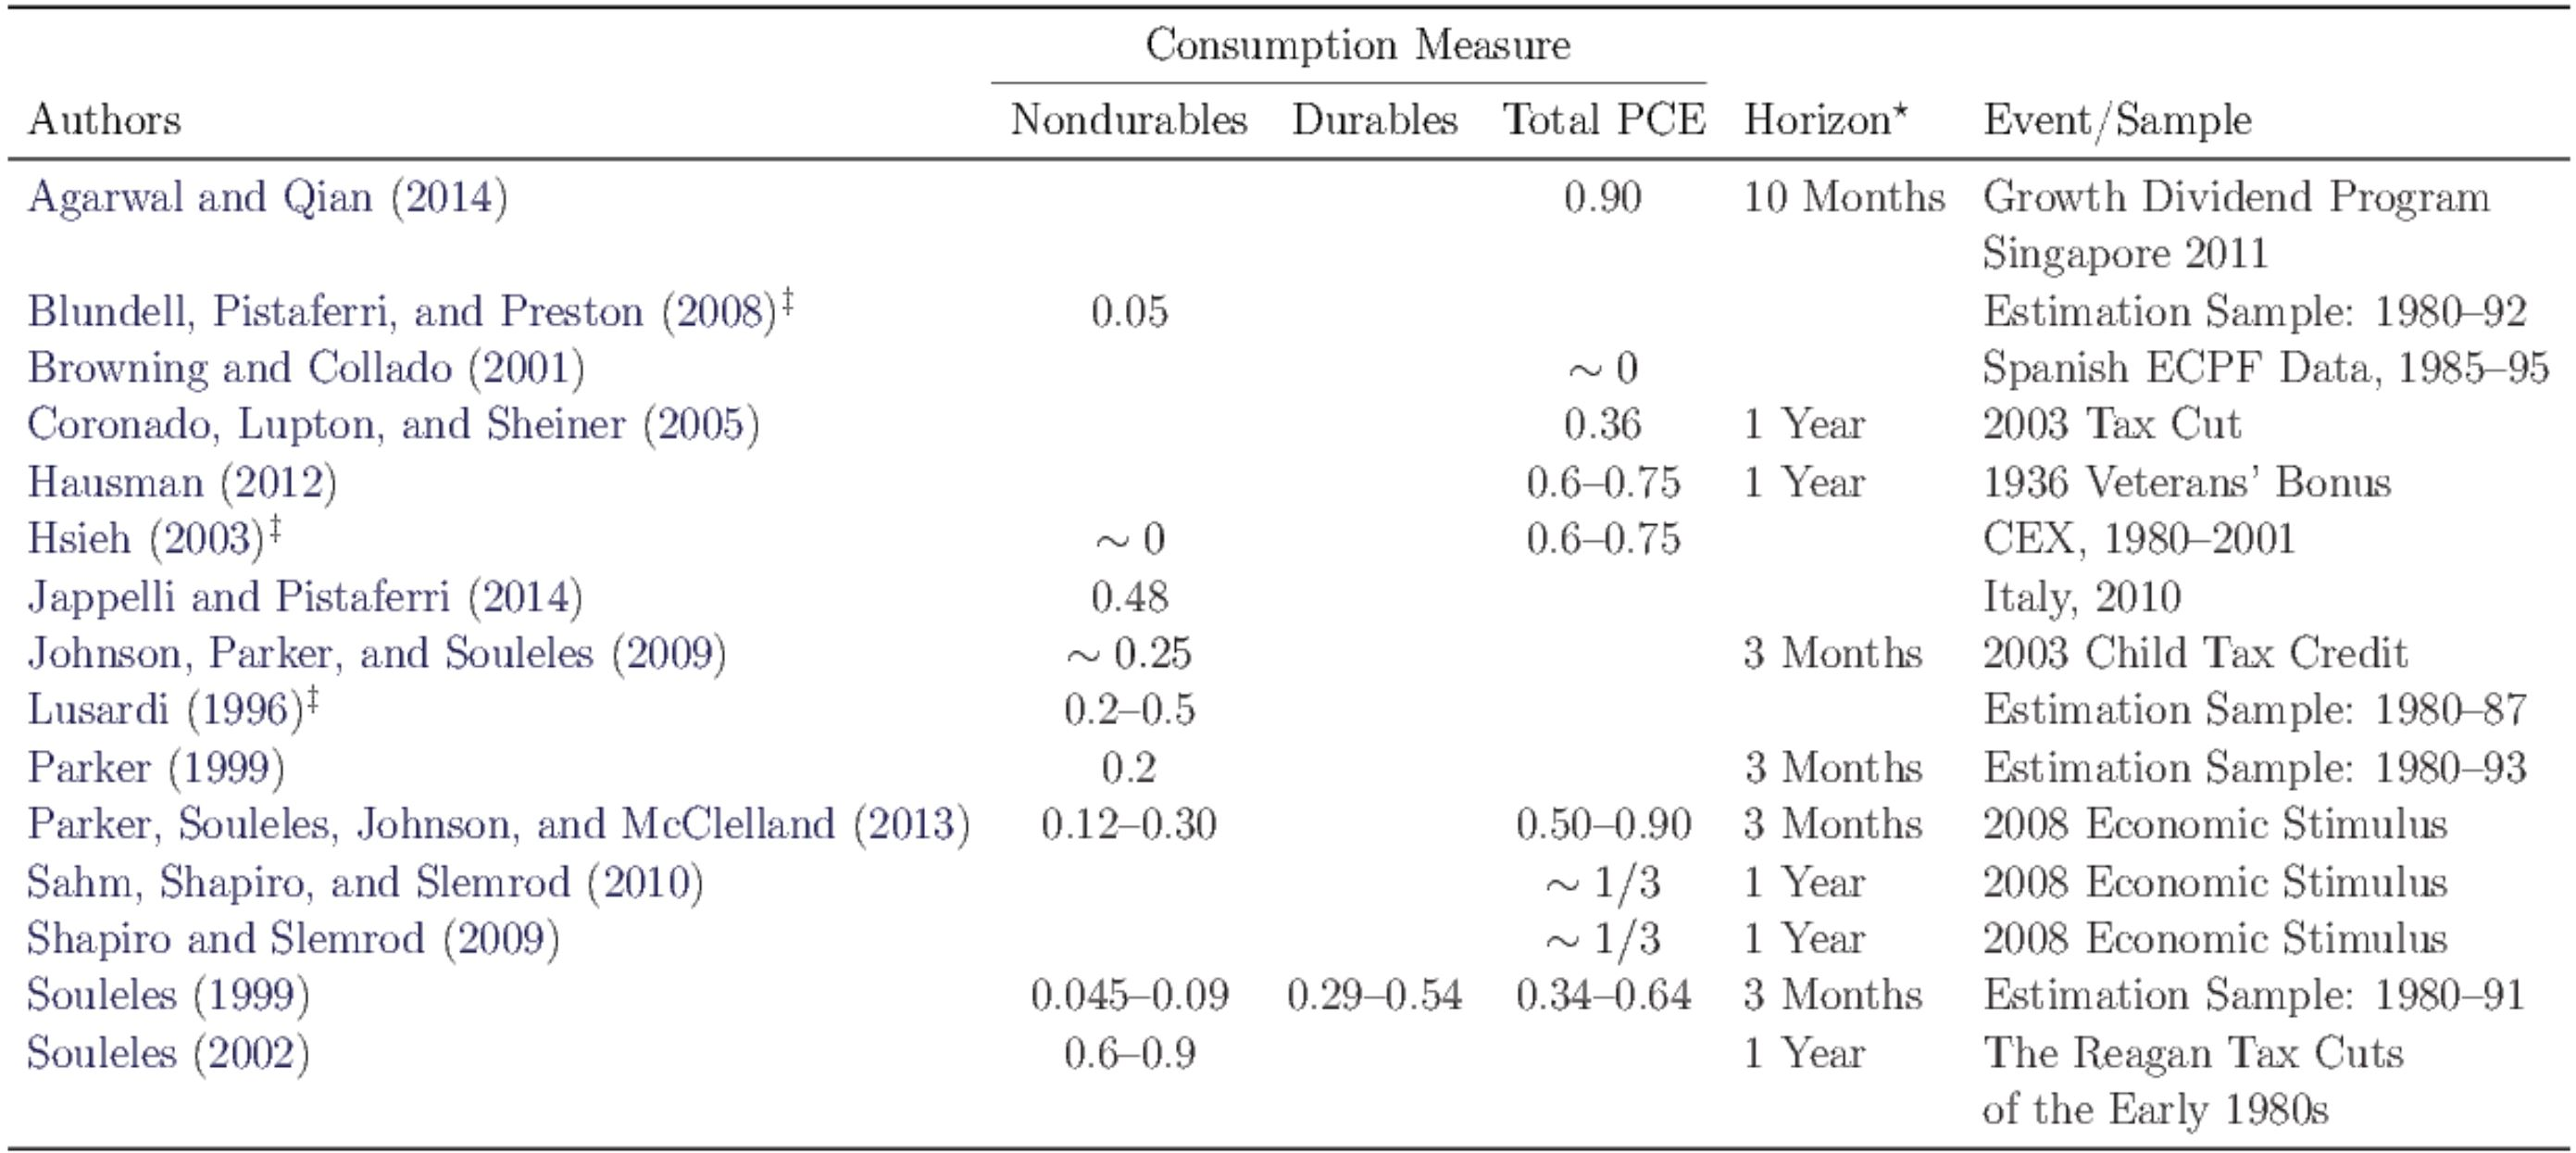
\includegraphics[scale=0.5]{\econtexRoot/Figures/MPCEmpiricalTable.JPG}
		\caption{Table from \cite{carroll_distribution_2016}}
		\label{fig:MPCtable}
	\end{centering}
\end{figure}

The second method is to make use of subjective expectations, possibly combined with realized outcomes, about income and consumption. The most direct of these studies simply asks individuals how much of a transitory income change they would consume, as was done in the Italian Survey of Household Income and Wealth in 2010 and the NY Fed's Survey of Consumer
Expectations in 2016-2017. \cite{jappelli_fiscal_2014} find an aggregate MPC of 0.48 using this Italian data and are able to identify clear differences across levels of liquid wealth. \cite{fuster_what_2018} find a lower aggregate MPC in the NY Fed's survey, but find heterogeneity by both size a sign of the shock. While this method holds great promise, it is clearly limited by the accuracy of households' own response to the question.

The third method is to impose covariance restrictions on panel data of income and consumption and use these to identify the consumption response to income shocks of differing persistence. The most well known of these is the paper by \cite{blundell_consumption_2008} which uses imputed non-durable consumption data based on food expenditure reported in PSID data. They find very little consumption response to transitory shocks. We will use this method as a starting point and will explore it in more detail in section \ref{empirical_strategy}.

For a more complete overview of the literature on consumption responses to income changes, see \cite{jappelli_consumption_2010}. Figure \ref{fig:MPCtable} from \cite{carroll_distribution_2016} shows the range of estimates available in the literature. As well as different identification methods, the statistics reported differ in the time period over which the MPC is measured, as well as the inclusion of durable goods in the measure. Estimates that include durable goods tend to be significantly larger than those for non-durables.

The attempt by \cite{auclert_monetary_2015} to quantify his sufficient statistics for monetary policy transmission demonstrates how the literature could greatly benefit from better empirics on the marginal propensity to consume. He identifies the distribution of MPC across individuals with different interest rate exposure to be a particularly important feature of the monetary policy transmission mechanism. Intuitively if households with large variable rate mortgages have higher MPCs than the households that have lent to them, then a decrease in short term interest rates will redistribute wealth from the low MPC group to the high MPC group resulting in a increase in aggregate demand. Figure \ref{fig:Auclert} shows how far the empirics are behind the theory in this respect. The figure exhibits the best estimates available from each of the three methods of the MPC (y-axis) against unhedged interest rate exposure (x-axis). The left panel uses the self reported MPCs in the Italian data, the center panel makes use of the BPP methodology using PSID data and the right panel follows the \cite{johnson_household_2006} study of 2001 tax rebates. Not only are the average levels of MPCs very different in each of the three studies, the standard errors are very large and there is no agreement on the steepness of the gradient across unhedged interest rate exposure.
	\begin{figure} 
	\begin{centering}
	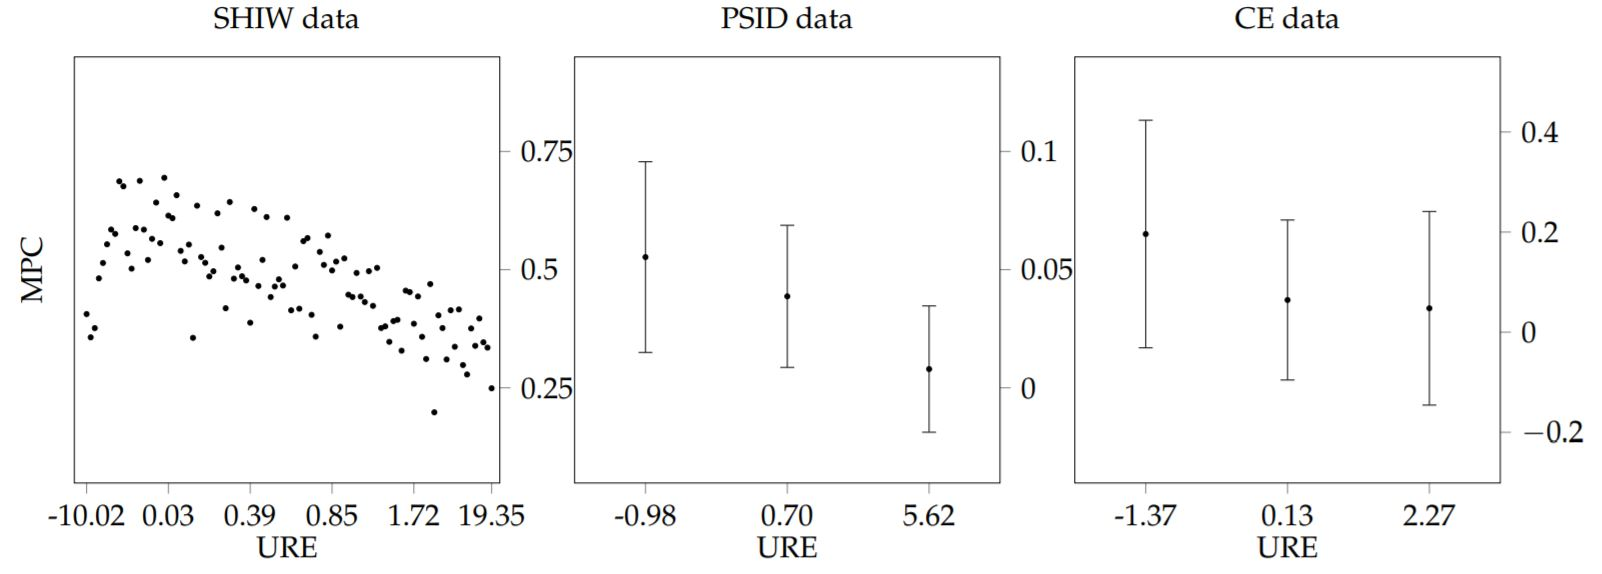
\includegraphics[scale=0.7]{\econtexRoot/Figures/MPCDistributionAuclert.JPG}
	\caption{Figure from \cite{auclert_monetary_2015}}
	\label{fig:Auclert}
	\end{centering}
	\end{figure}
	
\section{Preliminary Evidence on the Nature of Expenditure Responses to Income Changes}
In section \ref{empirical_strategy} we use a model to estimate the expenditure elasticities to transitory and permanent shocks and find surprisingly little difference between the two. While the model allows us to precisely estimate these quantities, in some ways it obscures from the key features of the data that are driving the result. In this section we present a some very simple regression of expenditure growth on income growth and compare them with what we would expect in some very well understood baseline models.

We will look at the estimate of $\beta^n$ in the model
\begin{align*}
    \Delta^n c_{it} = \alpha^n + \beta^n y_{it} + \varepsilon_{it}
\end{align*}
where $n$, the number of years over which growth is measured, varies from 1 to 10. Figure \ref{fig:GrowthReg} shows the resulting estimates for all Danish households whose head is between the age of 35 and 60 in 2013 (the sample covers 2003-2015). The striking feature, which drives our main results in section \ref{results}, is that $\beta^n$ is more or less constant across different values of $n$. To build intuition on why this result is so striking, we have also included the expected values of $\beta^n$ from simulating well understood models. The blue line shows the complete markets case where all idiosyncratic shocks can be, and are, insured against. The green line shows behavior from the Solow model in which households save a constant proportion of their income each period. The coefficients are equal to 1 even when saving is positive because we are looking at elasticities. Finally, the green line shows the expected result from a standard buffer stock savings model as described in section ***********. In this model, the variance of income growth over one year is dominated by the transitory shocks for which the consumption response is relatively small. Over a 10 year period the variance of income growth is dominated by permanent shocks to income, for which consumption moves close to one-for-one. As a result, this model gives rise to an upward sloping curve for $\beta^n$ asymptoting towards 1.

In the following section we will make specific assumptions about the income and consumption processes that allow us to identify the consumption elasticity to permanent and transitory shocks. We will also test the model for a variety of ways in which it may be misspecified. In all cases the conclusion that there is little difference between the permanent and transitory elasticities is robust. Intuitively, this fact can be traced back to the lack of an upward slope in the graph of $\beta^n$ above and this helps to guide thinking on alternative possible models.
	\begin{figure} 
	\begin{centering}
	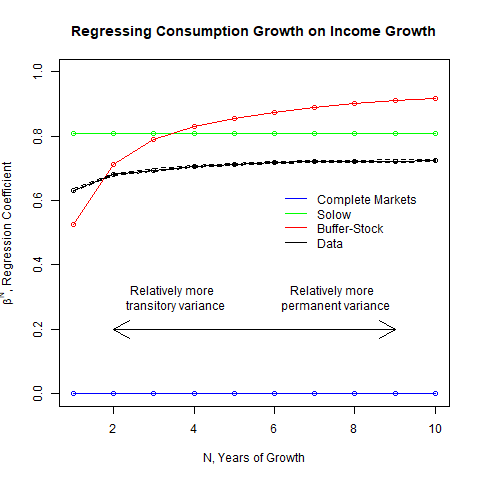
\includegraphics[scale=0.7]{\econtexRoot/Figures/basic_regression.png}
	\caption{Regression coefficients of consumption growth on income growth}
	\label{fig:GrowthReg}
	\end{centering}
	\end{figure}
	
\section{Empirical Strategy} \label{empirical_strategy}
Our methodology builds heavily on both \cite{blundell_consumption_2008} (BPP) and \cite{carroll_nature_1997}. The BPP framework has become a workhorse in the heterogeneous agent literature. \cite{kaplan_how_2010} show that the method gives reasonably accurate estimates in simulated data for a variety of realistically calibrated heterogeneous agent models and end up concluding ``The BPP insurance coefficients should become central in quantitative macroeconomics''. It has been somewhat of a mystery how the estimated BPP consumption response to transitory shocks (around 5\%) can be reconciled with much higher estimates from the natural experiment literature. \cite{commault_how_2017} is one attempt to explain this difference by allowing consumption growth to depend on the history of income shocks. We show that the time aggregtion problem, ignored in BPP and the simulation exercises of \cite{kaplan_how_2010}, significantly effects the identification and can explain the entire dissonance.

Once we correct for the time aggregation problem, it is apparent that the identification of transitory and permanent shock variance is very sensitive to the exact assumptions made about the short term dynamics of income. There is no clear way to adapt the MA process for transitory shocks assumed in BPP to our time aggregated framework. Instead we turn to the large literature on estimating transitory and permanent shock variances and in particular make use of \cite{carroll_nature_1997}. We follow their method of estimating permanent and transitory income shock variance using income growth over 3 to 5 years and extend it to consumption.
\subsection{The Time Aggregation Problem}
\cite{working_note_1960} was the first to note that if the observation period is longer than the underlying process and we observed the sum (or mean) of a random walk over the observation period, then the resulting observed process in not a random walk and has a positive autocorrelation. Intuition on this can be gained from figure \ref{fig:TimeAgg}. Here the underlying process (thin black line) is a random walk in continuous time while the observed process (think red line) is the mean of the underlying process over each time period. If a shock to the underlying process happens half way through a time period the expected value of the process will jump by the full amount of the shock, but the mean value observed in the current period will only jump by half the value of the shock. Therefore an increase in the time aggregated process in the current period is predictive of another increase in the next period. Consider the time period from 4 to 5 in figure \ref{fig:TimeAgg}. In this period the underlying process increases substantially from around -5 to 5. However, we only observe the time aggregate process increase by about half this amount, with the rest of the increase occuring in the following period despite the fact that the underlying process does not increase in the following period. If the underlying process is a random walk in continuous time (possibly with jumps), the first autocorrelation is 1/6 and the autocorrelation beyond one period is 0.
	\begin{figure} 
	\begin{centering}
		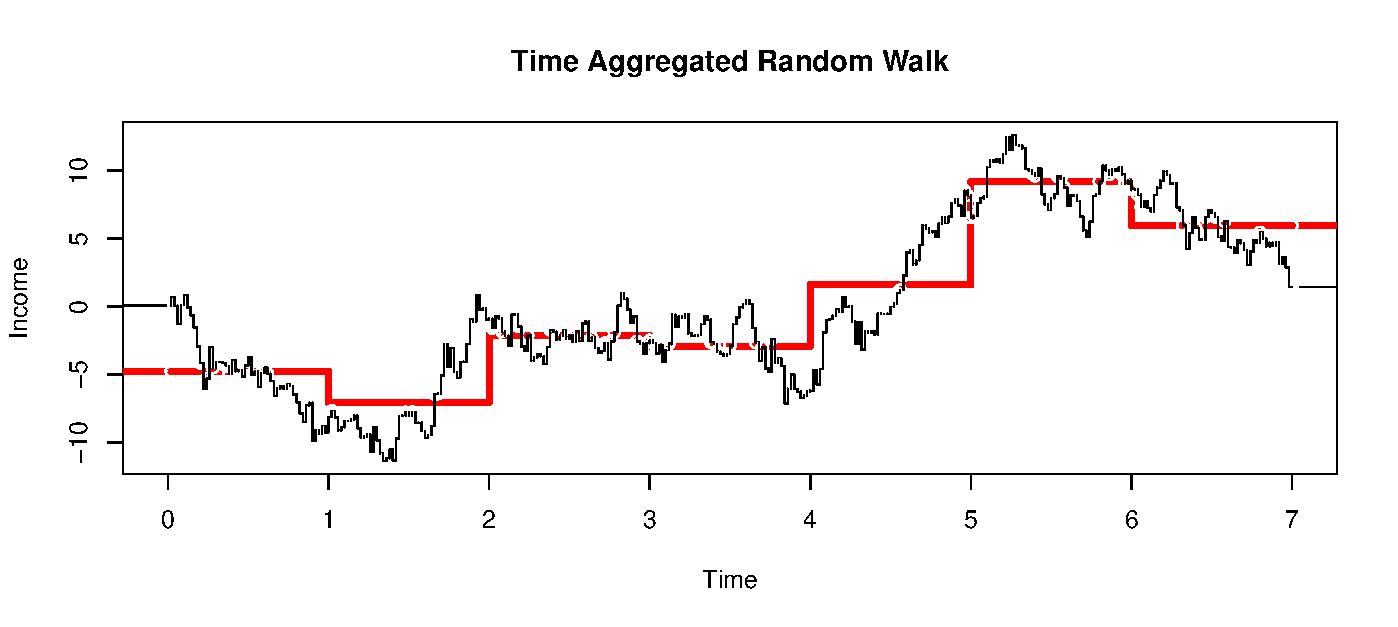
\includegraphics[scale=0.7]{\econtexRoot/Figures/timeagg_rw.pdf} 
		\caption{Time Aggregated Random Walk}
		\label{fig:TimeAgg}
	\end{centering}
\end{figure}
The time aggregation problem has mostly been absorbed by macroeconomists, for example \cite{campbell_consumption_1989} use two lags of the growth predicting instruments to overcome the problem. The household finance literature appears to have mostly ignored the problem, including all studies that use microdata to identify transitory and permanent shock variances. For some applications, including BPP, this oversight fundamentally changes the econometric results. In sections \ref{BPP_noagg} to \ref{BPP_cont} we describe the core BPP identification and then show how time aggregation affects the results with time aggregated over two periods and then in continuous time.

\subsubsection{BPP Identification without Time Aggregation} \label{BPP_noagg}
Below we summarize the BPP assumptions and derive the key moments used for identification. For a more detail please refer to their original paper. The core of the model is the assumptions on the income and consumption processes. They assume that (unexplained) income growth for household $i$ follows the process:
\begin{align*}
\Delta y_{i,t} = \zeta_{i,t} + \Delta \varepsilon_{i,t}
\end{align*}
where time is discrete and $\zeta_{i,t}$ and $\varepsilon_{i,t}$ are each i.i.d. and independent of each other.\footnote{BPP allow the transitory component to follow an MA(q) process. As our purpose here is simply to demonstrate the importance of time aggregation in this application, we consider the simplest version. The core idea is unchanged by the inclusion of MA(q).} The (unexplained) change in log consumption is assumed to be:
\begin{align*}
\Delta c_{i,t} = \phi_{i,t}\zeta_{i,t} + \psi_{i,t} \varepsilon_{i,t}
\end{align*}
That is consumption follows a random walk as proposed in \cite{hall_stochastic_1978}. $\phi_{i,t}$ can be thought of as being closely related to the MPC out of permanent shocks and $\psi_{i,t}$ closely related to the MPC out of transitory shocks.\footnote{Strictly these coefficients are elasticities. They are closely related to their respective MPCs because for many households, total consumption is close to total income, so a one percentage point increase in consumption corresponds to one percentage point of income.}

Identification of $\psi$ is achieved by noting that predictability in income growth comes only from the transitory component of income (which is mean reverting) while the permanent component of income contains no information about future income growth. Therefore income growth in the next period acts as a valid instrument for $\varepsilon_{i,t}$.
\begin{align}
\psi &= \frac{\mathrm{Cov}(\Delta c_t,\varepsilon_t)}{\mathrm{Cov}(\Delta y_t,\varepsilon_t)} \nonumber \\
&= \frac{-\mathrm{Cov}(\Delta c_t,\Delta y_{t+1})}{-\mathrm{Cov}(\Delta y_t,\Delta y_{t+1})} \label{tran_ins}
\end{align}
An estimate of the right hand side of equation \ref{tran_ins} can be calculated from the sample and is used to identify $\psi$.

\subsubsection{BPP Identification with Two-period Time Aggregation} \label{BPP_two_period}
Here we show the identification problem that arises when the underlying process is made up of two sub-periods (we will assume of 6 months each), but we observe the sum of income and consumption of the whole year. As before the underlying processes for income and consumption growth are:
\begin{align*}
\Delta y_t & = \zeta_t + \Delta \varepsilon_t \\
\Delta c_t & = \phi \zeta_t + \psi \varepsilon_t  \\
\end{align*}
where now $t$ denotes 6-month periods. Summing up (assuming $y_0=c_0=0$) gives:
\begin{align*}
y_t & = \sum_{i=1}^t \zeta_i + \varepsilon_t  \\
c_t & = \phi \sum_{i=1}^t \zeta_i + \psi \sum_{i=1}^t \varepsilon_i  \\
\end{align*}
We observe $y^{obs}_T$ and $c^{obs}_T$ for $T \in \{2,4,6...\}$ (annually) where:\footnote{Here we are being a little fast and loose by summing the log process rather than actual income process. We will continue to do this throughout the paper. In appendix \ref{sec:Identification} we show do this properly, making the assumption that the variance of permanent income over a one year period is small.}
\begin{align*}
y^{obs}_T & = y_T + y_{T-1}  \\
c^{obs}_T & = c_T + c_{T-1}  \\
\end{align*}
Our observed (annual) changes in income and consumption are therefore:
\begin{align*}
\Delta^2 y^{obs}_T & \equiv y^{obs}_T-y^{obs}_{T-2} =  y_T + y_{T-1} - y_{T-2} - y_{T-3} \\
\Delta^2 c^{obs}_T & \equiv c^{obs}_T-c^{obs}_{T-2} =  c_T + c_{T-1} - c_{T-2} - c_{T-3}  \\
\end{align*}
which implies:
\begin{align*}
\Delta^2 y^{obs}_T & = \zeta_T + 2\zeta_{T-1} +\zeta_{T-2} + \varepsilon_T + \varepsilon_{T-1} - \varepsilon_{T-2} - \varepsilon_{T-3} \\
\Delta^2 c^{obs}_T & =  \phi(\zeta_T + 2\zeta_{T-1} +\zeta_{T-2}) + \psi(\varepsilon_T + 2\varepsilon_{T-1} + \varepsilon_{T-2} ) \\
\end{align*}
Following the BPP method we would now use these observed growth numbers in the identification equation \ref{tran_ins}. This results in the value:
\begin{align}
\frac{-\mathrm{Cov}(\Delta^2 c^{obs}_T,\Delta^2 y^{obs}_{T+2})}{-\mathrm{Cov}(\Delta^2 y^{obs}_T,\Delta^2 y^{obs}_{T+2})} &= \frac{\phi \mathrm{Var}(\zeta_T) -\psi(\mathrm{Var}(\varepsilon_T) + 2\mathrm{Var}(\varepsilon_{T-1}) )}{ \mathrm{Var}(\zeta_T) - \mathrm{Var}(\varepsilon_T) -\mathrm{Var}(\varepsilon_{T-1}) } \nonumber\\
& = \frac{\phi \mathrm{Var}(\zeta_T) -3\psi \mathrm{Var}(\varepsilon_T)  }{ \mathrm{Var}(\zeta_T) - 2\mathrm{Var}(\varepsilon_T)  }	\label{psihat}
\end{align}
which bears little relation to the desired value of $\psi$. For example, if the underlying consumption process followed the permanent income hypothesis with $\phi=1$ and $\psi=0$, and transitory shock variance was the same size as permanent shock variance, the expected value of the estimate for $\psi$ would be $-1$!

\subsubsection{BPP Identification with Time Aggregation in Continuous Time} \label{BPP_cont}
By now it should be clear that time aggregation is a serious problem for the BPP method. A natural question arises as to what frequency of underlying process to use to best approximate households' actual income processes. It is important to distinguish between a model in which shocks happen about once a year (for example) but can occur at any point in the year, versus a model in which shocks to income happen on a timetable, say on 31st December each year. The former can be modeled in continuous time with jumps occurring as a Poisson process approximately once a year. The later is best modeled as a discrete time model as the original BPP paper. In this paper we will take the former approach. While some types of jobs may have a regular schedule on which pay appraisals take place, our evidence suggests that most of the variance in both transitory and permanent income is relatively evenly spaced throughout the year.\footnote{We will soon have access to monthly pay data which will allow for a more rigorous analysis of this assumption.} Many of the larger permanent shocks to income occur when a worker changes job which can occur at any point in the year. We (along with the literature) lack a clear understanding of what makes up the bulk of the transitory shocks to income, but regularly scheduled bonuses are not large enough to account for much of this variance. Furthermore, even if each individual household experienced shocks on a pre-set timetable, if the timetable itself varies across the year for different households, our approach would yield unbiased results. While there is a big change in going from an underlying annual process to a quarterly process, the further change from quarterly to continuous time is much smaller. As the exposition is much simpler in continuous time, we will therefore chose to present our own method in continuous time.

To write the equivalent model including purely transitory and permanent shocks in continuous time we will define two underlying martingale processes (possibly with jumps), $P_t$ and $Q_t$ where $P_t$ is the \textit{flow} of permanent income at time $t$ and $Q_t$ is the \textit{sum} of transitory shocks up to time $t$. We assume that for all  $s_1>s_2>s_3>s_4>0$:
\begin{align*}
\mathrm{Var}(P_{s_1}-P_{s_2})=(s_1-s_2)\sigma_P^2 \\
\mathrm{Cov}(P_{s_1}-P_{s_2},P_{s_3}-P_{s_4}) = 0 \\
P_s = 0 \qquad \text{if } s<0
\end{align*}
and similarly for $Q_t$. Instantaneous income in a period $dt$ is given by:
\begin{align}
dy_t = \Big( \int_{0}^{t}dP_s \Big) dt  +dQ_t \label{income_process}
\end{align}
so that $P_t$ and $Q_t$ are exactly analogous to the permanent and transitory shocks in the discrete time model (with $q=0$ in the MA($q$) transitory component). Keeping with the assumption that consumption is a random walk with response parameters $\phi$ and $\psi$, instantaneous consumption is given by:
\begin{align}
dc_t = \phi \Big( \int_{0}^{t} dP_s  \Big) dt +\psi\Big( \int_{0}^{t}dQ_s\Big) dt  \label{consumption_process}
\end{align}
Equations \ref{income_process} and \ref{consumption_process} give the instantaneous income and consumption process in continuous time. We do not observe instantaneous quantities but instead the time aggregated quantities:
\begin{align}
\bar{y}_T = \int_{T-1}^{T} dy_t \label{income_TA}\\
\bar{c}_T = \int_{T-1}^{T} dc_t \label{cons_TA}
\end{align}
for $T \in \{1,2,3...\}$. Taking the first difference gives:
\begin{align}
\Delta \bar{y}_T &= \int_{T-1}^{T} dy_t  - \int_{T-2}^{T-1} dy_t  \nonumber \\ 
&= \int_{T-1}^{T} \int_{0}^{t}dP_s dt -\int_{T-2}^{T-1} \int_{0}^{t}dP_s dt +  \int_{T-1}^{T} dQ_t -\int_{T-2}^{T-1} dQ_t \nonumber \\
&= \int_{T-1}^{T} \int_{t-1}^{t}dP_s dt +  \int_{T-1}^{T} dQ_t -\int_{T-2}^{T-1} dQ_t \nonumber \\
&= \Big(\int_{T-2}^{T-1} (s-(T-2))dP_s  + \int_{T-1}^{T} (T-s)dP_s \Big) \nonumber \\
& \qquad + \Big(\int_{T-1}^{T} dQ_t -\int_{T-2}^{T-1} dQ_t \Big) \label{deltay}
\end{align}
and a similar equations for $\Delta \bar{c}_T$. Putting these observable income and consumption changes into the identification equation \ref{tran_ins} gives:
	\begin{align}
	\frac{-\mathrm{Cov}(\Delta \bar{c_t}, \Delta \bar{y}_{t+1})}{-\mathrm{Cov}( \Delta \bar{y}_t, \Delta \bar{y}_{t+1})}
	&= \frac{ \frac{1}{6}\phi \sigma^2_P - \frac{1}{2}\psi \sigma^2_Q}{ \frac{1}{6} \sigma^2_P -  \sigma^2_Q} \label{psi_cont}
	\end{align}
As in the two sub-period example, it is clear that this equation does not identify $\psi$. It is a little easier to get intuition on exactly why here. First, the $\frac{1}{6} \sigma^2_P$ comes directly from the fact that a random walk in continuous time has a first autocorrelation of 1/6. Second the 1/2 in the numerator attached to the transitory variance comes from the fact that while all the income from a transitory shock arrives in the observed period, on average this will happen half way through a period so only 1/2 the annual consumption response will occur in that period.

\subsection{Our Empirical Strategy: Identification from Growth over 3, 4 and 5 years}
We could press ahead and use the same model, corrected for time aggregation, to identify the parameters of interest. However, we believe this would result in serious misspecification problems. In particular the assumption that consumption is a random walk becomes much important once time aggregation is corrected. \cite{kaplan_how_2010} show that in a model with no time aggregation, the BPP method identifies the contemporaneous spending response to a transitory shock regardless of consumption dynamics going forward. With time aggregation this is no longer the case and the spending response of an impatient consumer who spends a significant proportion of a transitory income shock in the first 3 months will be poorly identified. Most empirical evidence suggests that many households respond to a transitory income shock with a large initial spending boost, but that after a few years there is no measurable sustained increase in consumption. In contrast to BPP, we will make the assumption that the consumption response to transitory shocks is short-lived. This will allow us to identify how transitory income and transitory consumption co-move while maintaining flexibility on the exact shape of these impulse responses in the short run.

Our method will look like a combination of \cite{carroll_nature_1997}, who use income growth over 3, 4 and 5 years to identify the size of permanent and transitory shock  variances, and BPP in that we will extend this identification to consumption.

\subsubsection{\cite{carroll_nature_1997} Income Variance Identification}
First we will examine the empirical strategy of \cite{carroll_nature_1997} and correct it take account of time aggregation. \cite{carroll_nature_1997} make exactly the same assumptions about the income process as BPP. In the case where the transitory shock is allowed to be an MA(2) process this is:
	\begin{align*}
	y_t &= p_t + \varepsilon_t + \theta_1 \varepsilon_{t-1} + \theta_2 \varepsilon_{t-2} \\
	p_t &= p_{t-1} +\zeta_t\\
	\end{align*}
from which we can calcuate the variance of growth over $n \geq 3$ years :
	\begin{align}
	\mathrm{Var}(\Delta^n y_t) &= n \mathrm{Var}(\zeta) + 2\underbrace{(1+\theta_1^2 + \theta_2^2)\mathrm{Var}(\varepsilon)}_\text{``Total'' transitory variance} \qquad \text{ for $n \geq 3$} \label{CS_identification}
	\end{align}
Equation \ref{CS_identification} shows that the variance of income growth grows linearly with the number of years of growth beyond 3. The transitory component adds variance at the beginning and end of the growth period, but any transitory shock to income that occurs in the middle of the period does not affect income growth as it will have died out by the end. \cite{carroll_nature_1997} use this to identify the variance of permanent shocks ($\mathrm{Var}(\zeta)$) and the ``total'' transitory variance ($(1+\theta_1^2 + \theta_2^2)\mathrm{Var}(\varepsilon)$). While similar to BPP it is important to note that BPP attempts to identify the variance of initial impact of the transitory shock, $\mathrm{Var}(\varepsilon)$, rather than the ``total'' transitory variance. While the notion of ``total'' transitory variance will carry over naturally into the time aggregated case, the variance of the initial impact does not have a natural interpretation.

The natural generalization of the MA(2) process in the case where the underlying income process has a higher frequency is to allow for an MA process with lags out to two years (so for a quarterly process this would be 8 lags etc). We find again that continuous time provides the most succinct and intuitive formulas. In continuous time we will allow for the impulse response to a transitory income shock to follow any generic path, $f(t)$, as long as it has died by two years after the shock ($f(t)=0 \quad \forall \quad t \geq 0$). An example of such impulse response can be seen in figure \ref{fig:GenericTransitory}, in this case the transitory shock lasts less than 1 year. In this model the flow of income is given by the sum of income arising from permanent income and any transitory shocks to income that have occurred in the previous 2 years:
	\begin{figure} 
	\begin{centering}
		\includegraphics[scale=0.7]{\econtexRoot/Figures/GenericTransitory.png} 
		\caption{Generic Transitory Shock Impulse Response}
		\label{fig:GenericTransitory}
	\end{centering}
\end{figure}
\begin{align*}
y_t &= \int_{0}^{t} dP_s + \int_{t-2}^{t} f(t-s)dQ_s
\end{align*}
Defining time aggregated income as in equation \ref{income_TA}, the variance of time aggregated income of an $n$ year period is:
	\begin{align}
\mathrm{Var}(\Delta^n \bar{y}_T) &= (n-\frac{1}{3})\sigma^2_P +  2 \mathrm{Var}(\tilde{y}) \text{   for }n \geq 3 \label{variance}
\end{align}
This is similar to the non time aggregated case (equation \ref{CS_identification}) except the coefficient on permanent variance is $n-\frac{1}{3}$. This error, though having less serious consequences than for BPP, has nevertheless been overlooked by the large literature that studies income dynamics using panel data.\footnote{For examples see \cite{moffitt_trends_2012}, \cite{meghir_income_2004}, \cite{nielsen_impact_2004}, \cite{heathcote_unequal_2010} and more recent quantile regression approaches such as \cite{arellano_earnings_2017}.} As with the MA(2) case the transitory variance identified is the variance of ``total'' transitory income received in the year, $\tilde{y}$, where this is defined as:
\begin{align}
\tilde{y_T} = \int_{T-1}^{T}\int_{t-2}^{t} f(t-s)dQ_s dt \label{tot_income}
\end{align}

\subsubsection{Extending \cite{carroll_nature_1997} to Consumption}
Our approach will be to extend the identification of income variance by using growth over 3, 4 and 5 years to also identify the covariance of income and consumption. In contrast to BPP, which assumes consumption follows a random walk, we will instead assume that the impulse response to a transitory shock follows a generic path, $g(t)$, that like the transitory income shock has fallen to zero two years after the news of the shock. Figure \ref{fig:GenericTransitoryBPP} shows possible paths for both income and consumption, along with the alternative random walk impulse response. In section \ref{misspecification} we will show why we think this two year time frame is empirically reasonable. We will maintain the assumption that the impulse response to a permanent shock to income follows a random walk. Under these assumptions the instantaneous flow of consumption is given by:
	\begin{align*}
c_t  &= \phi \int_{0}^{t}dP_s  + \int_{t-2}^{t} g(t-s)dQ_s  \\
\end{align*}
	\begin{figure} 
	\begin{centering}
		\includegraphics[scale=0.6]{\econtexRoot/Figures/GenericTransitoryConsumptionWithBPP.png} 
		\caption{Generic Transitory Shock Impulse Response}
		\label{fig:GenericTransitoryBPP}
	\end{centering}
\end{figure}
and the covariance of time aggregated income and consumption growth over $n \geq 3$ years is given by
	\begin{align}
\mathrm{Cov}(\Delta^n \bar{c_T},\Delta^n \bar{y_T} ) &= \phi (n-\frac{1}{3}) \sigma^2_p + 2 \mathrm{Cov}(\tilde{c},\tilde{y}) \text{  for  } n\geq 3 \label{covariance}
\end{align}
where total transitory income, $\tilde{y}$ is given by equation \ref{tot_income} and total transitory consumption, $\tilde{c}$, is defined by:
\begin{align}
\tilde{c_T} = \int_{T-1}^{T}\int_{t-2}^{t} g(t-s)dQ_s dt \label{tot_cons}
\end{align}
Using the equation for variance \ref{variance} and covariance \ref{covariance} of income and consumption growth over $n$ years for at least 2 different values of $n$, we are able to identify the 4 unknowns we are interested in:
	\begin{itemize}
	\item $\sigma^2_p$ Variance of permanent shocks
	\item $\mathrm{Var}(\tilde{y})$ Variance of transitory income received in a year
	\item $\phi$ Elasticity of consumption w.r.t permanent income
	\item $\psi = \frac{\mathrm{Cov}(\tilde{c},\tilde{y})}{\mathrm{Var}(\tilde{y})}$ Elasticity of transitory consumption w.r.t transitory income over a year
\end{itemize}
Our panel data covers 10 years and we choose to use growth over 3, 4 and 5 years to balance greater identification (longer growth periods give more power) with the fact that many households drop out of the sample if we demand they have reliable data for the too many consecutive years. Using growth over 3 different time periods means the system is over identified with 6 equations with which to estimate these 4 unknowns. We follow BPP and use diagonally weighted minimum distance estimation, although our results are not significantly changed by using other popular weighting methods.\footnote{In general our results may be subject to misspecification problems, but the sample size of our data means that standard errors are small.}

Of the four parameters identified we will be particularly interested in $\psi$ so it is worth thinking about exactly what this parameter represents. Casually we can think of this as a marginal propensity to consume out of transitory shocks, but more strictly the following description holds:

$\psi=0.7$ means \textit{``If income this year is 1\% higher than it would have been with no transitory shocks this year or in the last 2 years, then consumption is on average 0.7\% higher than it would have been''}

For households who consume close to their permanent income, this elasticity can be thought of in levels, so that $\psi=0.7$ means if transitory income is \$100 in a year, then consumption is on average \$70 higher than it would otherwise have been. For households (mainly very wealthy) who consume significantly less than their permanent income, this conversion to levels must be adjusted by the proportion by which consumption is less than permanent income.

\section{Data}
Our panel data on income and expenditure comes from Danish registry data from 2003-2015. This data has a number of advantages over survey based measures. First, the sample contains millions of households rather than thousands. Second, households are required by law to report their data so there is much less risk of selection bias through drop outs. Third, measurement error in income data is largely eradicated, as employees' income data is third party reported by their employer, compared to survey data where self reported income has been shown to be particularly unreliable for irregular income.\footnote{See \cite{david_income_nodate} for a survey of income measurement error issues in survey data.}

\subsection{Income} \label{income}
We are interested in income and consumption decisions at the household level. We define a household as having either one or two adult members. Two adults are considered to be in the same household if they are cohabiting and married or they are cohabiting and have children. In the panel data, an individual's household will change if he or she gets married or divorced leading to some selection bias given that we require households to survive for at least 5 years. Household income is defined as the sum of total income after tax for all members of the household. The tax reporting system in Denmark is highly automated and individuals bear little of the reporting burden. For employees income is reported by their employers and is thought to be highly accurate. The underground economy in Denmark is small. We remove business owners from the sample as their income may be less accurately reported, but more importantly, because the expenditure imputation method does not work well for them (see section \ref{cons_imputation}).

We work with the residual of log income after controlling for observable characteristics of households that may affect their income and consumption. To start we remove households in the top and bottom 1\% of the income distribution. We then regress log income on dummys for age, year, highest level of education, marital status, homeowner status and number of children along with interaction of age with education, marital status and homeowner status. We take the change in the residuals of this regression to be the unexpected income change for a household from one year to the next and remove households in the top and bottom 1\% of the unexpected income \textit{change} distribution.

\subsection{Imputed Expenditure} \label{cons_imputation}
Our expenditure data comes from imputing expenditure from income and wealth. Along with other Scandinavian countries, Denmark is unusual in that tax reporting includes information about wealth along with income, a legacy from the wealth tax that was phased out between 1989 and 1997. Following the methodology from \cite{browning_imputing_2003} and \cite{fagereng_imputing_2015} we impute expenditure using the identity:
		\begin{align*}
	\bar{C_t} \equiv \bar{Y_t} - \bar{S_t} = \bar{Y_t} - \Delta NW_t
	\end{align*}
where $\bar{C_t}$, $\bar{Y_t}$ and $\bar{S_t}$  are the sum of expenditure, income and savings over the year $t$ respectively. $\Delta NW_t$ is the change in net worth measured at the end of years $t$ and $t-1$. Banks and brokers are required to report the value of their clients' accounts on 31\textsuperscript{st} December each year, and the the tax reporting year runs from 1\textsuperscript{st} January to 31\textsuperscript{st} December, so the data for income and wealth reported in the tax returns matches with that required to use this identity to impute consumption.

The method works well for households with simple financial lives. One of the biggest problems with the method is its inability to handle capital gains well. The income used in the imputation includes all labor income and capital income, however it excludes capital gains. The value of assets will vary both due to savings from reported income but also due to capital gains and losses. We handle this in a number of ways. First, we completely exclude housing wealth from our measures of net worth and saving, treating housing as an off balance sheet asset. The problem with treating housing in this way is that we must exclude households in years in which they are involved in a housing transaction. For the self employed, it is also difficult to distinguish between expenditure and investment in their business, so we exclude all households who receive more than a trivial amount of their income from business ventures. Finally, households that hold significant equity investments are likely to see sizable capital gains and losses. We make a naive adjustment by making the assumption that they hold a diversified index of stocks. While this will likely lead to significant measurement error for these individuals, the concern is mitigated first by the fact that stock holding is much more unusual in Denmark than in the US for example. Only around 10\% of households hold any stocks, and for many of those stocks make up only a small proportion of their total wealth. Furthermore, as we will explain in section \ref{whysohigh}, measurement error in consumption is not a concern unless it is correlated with income. This seems unlikely to be the case, except for households that hold significant equity in the firms in which they work. Another concern with the imputation method is transfers of wealth, say between family members or friends. Indeed imputed expenditure is negative for approximately 3\% of households and this may explain a proportion of that. We throw out both income and expenditure data for households in years in which their expenditure is negative.

As with income, we work with the residual of expenditure after controlling for the same observable features as income. We follow exactly the same steps as described in section \ref{income}.

In evaluating how much we can learn from such a measure, it should be compared to the best alternatives available to economists. In the original BPP paper the authors only have access to food expenditures from the PSID data and impute total non-durable consumption by comparison with the Consumer Expenditure Survey. Self reported consumption is also notoriously poor quality even in comparison to self reported income. Furthermore, in the PSID data the questions in food expenditure are ambiguous as to which period exactly the question is referring to.

\subsection{Sample Selection}
As our methodology requires income uncertainty to be relatively constant through the observed period so we limit the sample to households headed by an individual between the age of 35 and 60. Section \ref{inc_variance} shows the assumption holds for this age group. Our final sample contains 23.3 million observations over 2004-2015, or approximately 1.9 million households per year.

\section{Results} \label{results}
Our results show:
\begin{itemize}
	\item Transitory and permanent income variance are approximately the same size for the population as a whole
	\item There is a lot of heterogeneity in the variance of permanent and transitory shocks, both in absolute and relative size
	\item The elasticity of income to permanent shocks is around 0.8
	\item The elasticity of income to transitory shocks is around 0.7, higher than most previous studies have found
	\item The expenditure response to transitory shocks is close to 1 for households with very little liquid wealth and drops to about 0.5 for the top quintile of households in liquid wealth.
	\item There is a similar, but less pronounced drop in the expenditure response to permanent shocks by liquid wealth.
\end{itemize}

\subsection{Income Variance} \label{inc_variance}
\begin{figure} 
\begin{centering}
	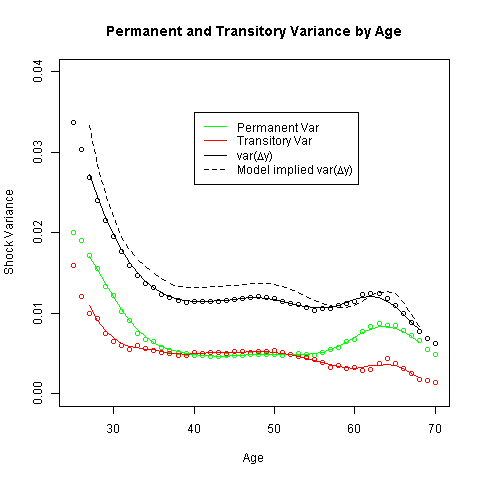
\includegraphics[scale=0.6]{\econtexRoot/Figures/VarianceByAge.png} 
	\caption{Permanent and Transitory Shock Variance by Age}
	\label{fig:VarianceByAge}
\end{centering}
\end{figure}
Figure \ref{fig:VarianceByAge} shows the computed permanent and transitory shock variances dividing the sample up into the age of the household head at the end of the sample period. The dots represent the minimum distance estimate for each age group while the lines are centered moving averages over the 5 nearest age groups. The solid black line shows the total variance of income growth over 1 year. It should not be surprising that income growth for households with heads in their 20's is highly volatile. This volatility plateaus around the age of 35 and stays at a constant level until the point of retirement at which point it temporarily grows before falling to an even lower level. We can see that while both transitory and permanent shocks to income are high early in life, permanent income shocks are particularly large while individuals find their place in the workforce. From the age of 35 to 60 both transitory and permanent shocks are approximately the same size and remarkably stable. At retirement shocks to permanent income rise, not surprisingly as retirement itself will be seen in the model as a shock, even as transitory income variance declines.

As the model assumes the variance to permanent and transitory shocks is constant in the observed period, interpretation of the numbers outside of the 35-60 age group needs to be treated with care. However, the figure clearly shows that within this age group the assumption of constant variance appears to be a reasonable one.

The dotted black line shows the variance of $\Delta y$ assuming no persistence in the transitory component. The fact that this line is slightly above the empirical variance of $\Delta y$ is consistent with some persistence in the transitory component of income, justifying our decision exclude growth over one and two years in our identification.

The level of both permanent and transitory shock variance for households aged 35 to 60 is approximately 0.006, reflecting a standard deviation of 8\%. Estimates using US data are significantly higher, especially for the transitory shock variance (for example \cite{carroll_nature_1997} estimate 0.02 for permanent and 0.04 for transitory). This difference may be due to lower income inequality in Denmark, more progressive taxation and more generous unemployment insurance. The lower transitory variance will also be due to significantly reduced measurement error relative to the survey based US data. 

\subsection{Consumption Response}
\begin{figure} 
	\begin{centering}
		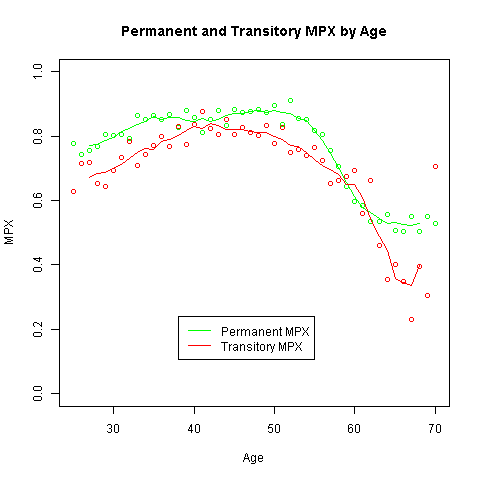
\includegraphics[scale=0.6]{\econtexRoot/Figures/MPXByAge.png} 
		\caption{MPX by Age}
		\label{fig:MPXByAge}
	\end{centering}
\end{figure}
Figure \ref{fig:MPXByAge} shows the model's estimates for $\psi$, informally labeled as the MPX (Marginal Propensity to eXpend). MPX out of permanent shocks remains relatively steady above 0.8 up to the head of household's early 50's (representing the 10 year's from the head's early 40's to early 50's) at which point it starts to fall. This is consistent with a lifecycle model in which a `permanent' shock to income represents a much smaller share of the household's lifetime budget constraint as retirement approaches. The MPX out of transitory shocks is notable for being high relative to other estimates in the literature, averaging around 0.7. It similarly declines towards retirement, but the decline starts earlier than the permanent MPX and is less steep. The pattern of this data is consistent with the majority of households acting as buffer stock savers in their early careers and then building up wealth as they approach retirement, giving them more room to smooth consumption. However, the magnitudes of the transitory MPX are larger than standard parameterizations of such models would imply.
\begin{figure}
	\centering
	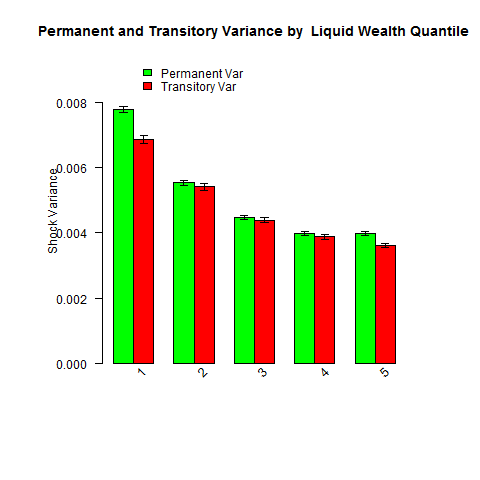
\includegraphics[scale=0.45]{\econtexRoot/Figures/VarianceByLiquidWealth.png}
	\centering
	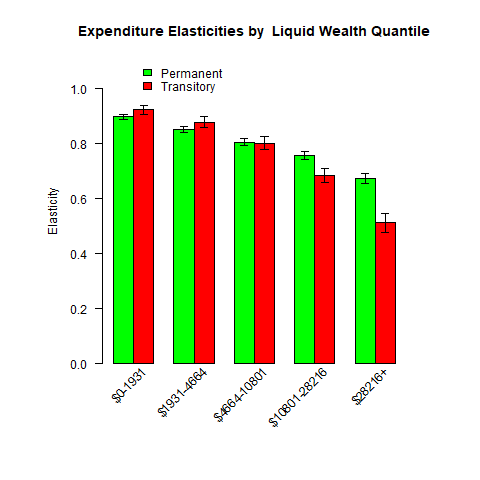
\includegraphics[scale=0.45]{\econtexRoot/Figures/MPXByLiquidWealth.png}
	\caption{Variance and MPX by Liquid Wealth Quintile}
	\label{fig:MPXByLiquidWealth}
\end{figure}

Figure \ref{fig:MPXByLiquidWealth} shows the model estimates for both permanent and transitory variance and MPX divided into liquid wealth groups. Households are first divided into groups according to the average level of liquid assets held over the sample period. The top quintile represents households that held an average of approximately \$50,000 or more in liquid assets, the middle quintile approimately \$10,000 and the bottom quintile held less than \$2000. The left panel shows that both permanent and transitory variance is higher for households with few liquid assets, possibly a reflection of the average age of these households. From the median quintile up the variance of income shocks stays at a relatively constant low level. The right panel shows that spending for households with high levels of liquid wealth is much less responsive to transitory income changes. While the MPX out of permanent shocks declines a little from 0.9 for the least liquid quintile to just under 0.8 for the top quintile, the MPX out of transitory shocks goes down from 0.9 to just above 0.5.

\subsection{Robustness to Misspecification} \label{misspecification}
In general the estimated permanent and transitory shock variance will be sensitive to the exact assumptions made about the income process. For example allowing the permanent component to mean revert (as in \cite{ahn_when_2017} or \cite{arellano_earnings_2017}) or allowing for correlation between the permanent and transitory shocks will affect how the total observed variance is divided between permanent and transitory. However, as the estimates we obtain for transitory and permanent MPX are close to equal to each other these results are relatively robust to different specifications of the income process.\footnote{We plan to carry out a number of robustness tests by changing the assumptions made about both the income and consumption processes. Our initial results suggest the estimated variances can change significantly, but the estimated MPX numbers are relatively robust.}

A key part of our identification method is the assumption that the impulse response for both income and consumption to a transitory shock has decayed to zero two years after the initial shock. We used growth over 3, 4 and 5 years for our identification because three years is the minimum to allow for generic impulse responses up to two years and demanding that households have more than five years of continuous data reduces the sample and possibly introduces sample selection problems. Figure \ref{fig:IncreasingDiff} makes use of the fact that our model is overidentified with the rich data available to us, so we can test some of this assumption. The solid black line shows the empirically measured variance of income growth over 1 to 7 years. The solid red line draws the straight line equation \ref{variance} with transitory and permanent variance parameters estimated using minimum distance on 3, 4 and 5 years of income growth. The empirical variance of income growth over two and three years is lower than this red line showing equation \ref{variance} is not valid for $n < 3$, consistent with some persistence in the transitory shock extending out to two years. However, the empirical variance over 6 and 7 years of income growth falls almost exactly on the red line implied by the model. This is strong evidence that the transitory component and income does not persist more than two years and that the permanent component does not mean revert at any significant rate.\footnote{We plan to carry out formal overidentification tests here. As we have so much data it is very likely that such a test suggest our model is misspecified. This would not be a concern (all models are simplifications) unless it is economically significant, something figure \ref{fig:IncreasingDiff} shows is not the case.}

The dashed black line and solid green line repeat this experiment with the covariance of income and consumption over increasing years of growth. This time the solid green line is equation \ref{covariance} with parameters identified by 3, 4 and 5 years of growth. As with income, the model says that this covariance should grow linearly for $n \geq 3$. The assumption that the transitory consumption response goes to zero within 2 years is less common than the equivalent assumption on income and is key to our identification. The data again show that for $n < 3$ the covariance is below the green line, but that for growth over 6 and 7 years the model does a good job.
\begin{figure} 
	\begin{centering}
		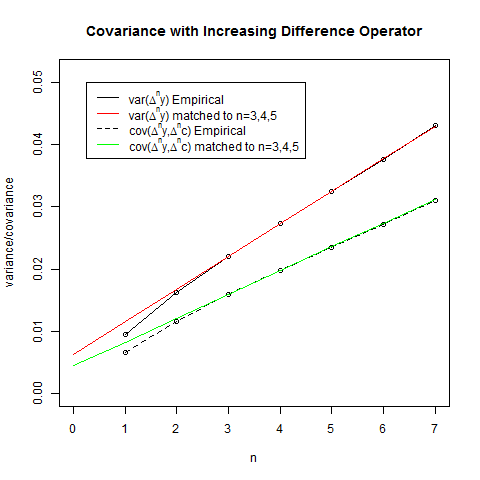
\includegraphics[scale=0.6]{\econtexRoot/Figures/IncreasingDiff.png}
		\caption{Variance and Covariance Over n Years of Growth}
		\label{fig:IncreasingDiff}
	\end{centering}
\end{figure}

\subsection{Why is the MPX out of Transitory Shocks so High?} \label{whysohigh}
The results of this paper for permanent shocks is generally in line with both theory and previous empirical work. However, the MPX out of transitory shocks is at the high end of empirical work and is especially high relative to standard consumption theory.

Figure \ref{fig:MPCtable} shows that our estimate of the MPX out of transitory shocks is at the high end, but not extreme. Our measure includes all spending on both durables and non-durables and represents the elasticity of consumption with transitory income received over a full year, a longer period than for many of the estimates in figure \ref{fig:MPCtable}. Estimates from \cite{agarwal_consumption_2014}, \cite{parker_consumer_2013} and \cite{souleles_response_1999} are all similar or higher than ours. However, \cite{fagereng_mpc_2016} estimate much lower MPXs (around 0.4) using well identified lottery winnings in a country (Norway) that is likely more similar to Denmark than the US. Furthermore, the expenditure data they use is imputed in a similar way to ours, so in order to take our results seriously we should have some idea why they may be so different to those from this paper. One answer may be that household's consumption response to a lottery win is different to other types of transitory shocks they may receive. While our initial impression is that households would spend more out of a lottery win (especially if they spend on celebrating the win), it is also possible that households put their winnings into a separate `mental account' (\cite{thaler_mental_1985}) from which they spend less than from their labor earnings. 

Another possibility, that deserves further investigation, is that our method may be picking up reverse causality between income and consumption. In our model, as is common in this literature, we treat the income process as exogenous. However, households may be able to adjust their labor supply in response to shocks. In particular, in years in which households have large spending needs (for example if they buy a car, carry out home improvements or pay for an offspring's wedding) it may be the case that they simultaneously increase their labor supply and hence earnings. Even (or especially) if the labor supply response is small, our model would see that as a very large increase in spending in response to a small increase in income. In future work we plan to address this in a quantitative model in which there are both transitory shocks to income and transitory shocks to consumption preferences. It is unclear to us at the moment how quantitatively important such a mechanism may be. Some empirical evidence that this mechanism may be important is that in households with two earners, the MPX out of transitory shocks from the secondary earner is significantly higher than for the primary earner. It is well established that the labor elasticity of secondary earners is higher than for primary earners so the possibility of reverse causality may be stronger for them.

A final possibility is that measurement error is driving our results to some extent. Our method is robust to classical measurement error in consumption. The permanent MPX is robust to classical measurement error in income while the transitory MPX would be biased downwards with classical measurement error in income uncorrelated with consumption. However, our method of imputing expenditure from income and wealth will pass any measurement error in income over to expenditure. Thus the portion of transitory income variance that is due to measurement error will have a related MPX of 1. Due to the fact that our income data comes from third party reported tax data we believe this portion is likely very small. We plan to investigate this by reducing the sample to households for whom we have reason to believe our income data is particularly accurate. We are also hoping to get access to monthly earnings data which will provide us with an independent source of income data, separate from that with which we imputed expenditure. A further test we plan to carry out is to use car purchases instead of total expenditure. This gives us a source of very well measured expenditure totally independent of our imputed expenditure method. This will act as a robustness test to our surprising result that even households with high levels of liquid wealth have expenditure tied closely with income.

\section{Models and Simulation}
What can these results tell us about the types of models typically used for modeling consumption behavior? Two natural questions arise:
\begin{itemize}
	\item How well does the econometric method work on standard incomplete market models?
	\item Can we calibrate a standard model to match the results we see, and if not are there changes we could make to the model that might help?
\end{itemize}
In this section we first introduce what is now the canonical buffer-stock savings model. We show that the econometric method is downward biased for the transitory consumption elasticity and upward biased for the permanent elasticity. When calibrated to the levels of transitory elasticity in the data, this bias is very small.
Motivated by the fact that, in the data, the consumption response to transitory shocks appears larger than much of the rest of the literature, we  build a model in which there is a reverse causality problem. We show that while the reverse causality can help to generate the high numbers we see for households with few liquid assets, the puzzle remains for households rich in liquid assets.

\subsection{The Standard Incomplete Markets Model} \label{standard_model}
Our baseline model is the now very familiar buffer-stock saving model of \cite{carroll_buffer_1997}. Given market resources ($\boldmath{\mLevBF}_t$), households in this model maximize expected utility:
\begin{align*}
	\mathbb{E}_t \sum_{i=t}^{\infty} \beta^i u(\cLevBF_i)
\end{align*}
subject to the constraints:
\begin{align*}
	\aLevBF_t = \mLevBF_t - \cLevBF_t \\
	\bLevBF_t = R\aLevBF_t \\
	\yLevBF_t = \theta_t \pLevBF_t \\
	\pLevBF_t = \Psi_t \pLevBF_{t-1} \\
	\mLevBF_t = \bLevBF_t + \yLevBF_t
\end{align*}
Where the felicity function, $u(\cLevBF)$ is CRRA. We will use this model to test the accuracy of our empirical method on simulated data. We chose two calibrations, presented in table *******. The first matches the distribution of liquid wealth in the economy, while the second is calibrated to more closely match the transitory consumption elasticity as measured in the data. In the first calibration, the economy is made up of agents with heterogenous discount factors following \cite{carroll_distribution_2016}. Agent $i$ has a discount factor $\beta_i$ where $beta_i$ is i.i.d across agents and follows a uniform distribution between $\beta_{low}$ and $\beta_{high}$. These two parameters allow us to match the fact that while the mean level of liquid assets is high, about to half of all households have close to zero liquid assets. Matching the lower part of this distribution is critical to generate transitory consumption elasticities substantially above zero. In the second calibration all the agents in the economy have the same discount rate. This is chosen to give a much higher transitory consumption elasticity, close to what we see in the data. To generate such a high elasticity it is necessary to introduce an unfeasibly low discount factor. In the following sections we will show how a model of this type could possibly be reconciled with the data.
Table \ref{table:simulation_psi} shows the estimates of $\psi$ using simulated data. The left hand panel shows the calibration to match the distribution of liquid assets. Here we see that using $n1=3$ and $n2=5$ underestimates the true elasticity, giving a value of 0.34 versus the `true' value of 0.38 obtained as $n1$ gets large (and hence the assumption that the consumption response lasts no longer that $n1-1$ years holds true). Thus, if this model was an accurate representation of the economy we would need to use a larger value of $n1$ or risk underestimating $\psi$. In the data we find our estimate for $\psi$ is in fact much \textit{larger} than implied by this model. In the second calibration the simulated estimate using $n1=3$ and $n2=5$, at 0.78, is very close to the `true' value of 0.79.
\begin{center}
	\input\econtexRoot/Tables/experimental/Psi_array2.tex	\input\econtexRoot/Tables/experimental/Psi_array1.tex
	\captionof{table}{Simulation estimates of $\psi$}
	\label{table:simulation_psi}
\end{center}
Table \ref{table:empirical_psi} shows how the estimate of $\psi$ varies when using different values of $n1$ and $n2$ in the data. The estimates around $n1$=3 and $n2$=5 are relatively stable at 0.76, but grow significantly as $n1$ increases beyond 5. This is likely due to the permanent shock in fact having some slow reversion to the mean that makes the method unreliable for larger values of $n1$. Appendix ****** shows that when permanent income follows an AR(1) process with persistence 0.95, the method is accurate for small values of $n1$ but becomes significantly upward biased as $n1$ gets large. This creates a tension between choosing $n1$ low enough to avoid this bias, but high enough such that we allow time for the consumption response to die and do not underestimate the coefficient.
\begin{center}
	\input\econtexRoot/Tables/experimental/Psi_array_empirical.tex		\captionof{table}{Empirical Estimates of $\psi$}
	\label{table:empirical_psi}
\end{center}
Table \ref{table:simulation_phi} shows the results of the simulation for the consumption elasticity to the permanent shock. Here we see very reliable estimates for any choice of $n1$ and $n2$ we care to make. Agents in the model adjust permanent consumption one for one with permanent income (in the medium run) and this comes through clearly in the estimates. The empirical counterpart to this, table \ref{table:empirical_phi}, also shows robustness to the choice of $n1$ and $n2$, apart from for larger values of $n1$. This is likely due to the same reason as the upward bias of $\psi$ for large $n1$, namely that the permanent shock is not entirely permanent.
\begin{center}
	\input\econtexRoot/Tables/experimental/Phi_array2.tex	\input\econtexRoot/Tables/experimental/Phi_array1.tex
	\captionof{table}{Simulation Estimates of $\phi$} 
	\label{table:simulation_phi}
\end{center}

\begin{center}
	\input\econtexRoot/Tables/experimental/Phi_array_empirical.tex		\captionof{table}{Empirical estimates of $\phi$}
	\label{table:empirical_phi}
\end{center}

\subsection{Preference Shock Model with Elastic Labor Supply} \label{pref_shock_model}
The empirical results of this paper suggest that the consumption response to a transitory shock to income lies at the high end of the existing literature. In this section we try to reconcile the results we get with the existing literature by asking if we can build a model in which our empirical method would estimate much larger elasticities than more traditional approaches to measuring the marginal propensity to consume out of transitory shocks. The intuition we build upon is that the households may wish to work longer hours, and hence earn more, in years when their expenditure is particularly high. If this were the case the income process would not be well modeled as being exogenous and our method would have a reverse causality problem embedded in it. Here we build such a model and see how much reverse causality can plausibly contribute to the results we obtain.
The model extends the standard incomplete markets model from section \ref{standard_model}, incorporating both preference shocks, so that households have some years when their utility of consumption is greater than others, and labor elasticity, so that households can adjust their income based on the marginal utility of consumption. The household's problem is to maximize expected lifetime utility:
\begin{align*}
\mathbb{E}_t \sum_{n=t}^{\infty} \beta^n \Bigg(\mathcal{X}_n \frac{ \cLevBF_n^{1-\rho}}{1-\rho}-\frac{\lLevBF_n^{1+\frac{1}{\xi}}}{1+\frac{1}{\xi}} \Bigg)
\end{align*}
subject to the constraints:
\begin{align*}
\aLevBF_t = \mLevBF_t - \cLevBF_t \\
\bLevBF_t = R\aLevBF_t \\
\yLevBF_t =  l_t w_t \\
\lLevBF_t = l_t \pLevBF_t^{\frac{1-\rho}{1+\frac{1}{\xi}}}\\
w_t = \theta_t \pLevBF_t \\
\pLevBF_t = \Psi_t \pLevBF_{t-1} \\
\mLevBF_t = \bLevBF_t + \yLevBF_t
\end{align*}
The normalization of labor $(\lLevBF_t = l_t \pLevBF_t^{\frac{1-\rho}{1+\frac{1}{\xi}}})$ is set up to allow labor supply to move elastically with transitory income, but the long run supply of labor does not depend on permanent income (as observed in the consistency of hours worked over long time periods and across countries). The key additional features of this model are i) the preference shock factor and ii) the elasticity of labor.

The preference shock factor, $\mathcal{X}_t$, multiplies the marginal utility of consumption in that period. When it is high the effective discount factor for consumption between this period and next is low so households will wish to spend much of their resources this period and will have little incentive to save for the next period. Equivalently when it is low, households will prefer to delay consumption to the following periods. There is little empirical evidence on the size of preference shocks, largely because consumption data usually has so much measurement error that estimating the standard deviation of consumption growth is very difficult. While a model with no preference shocks will normally imply a consumption path that is significantly smoother than the income process, our data suggests the standard deviation of income growth is 0.12 while the standard deviation of consumption growth is 0.37. Such a high standard deviation in consumption growth is likely to be mostly driven by measurement error on the asset side of the balance sheet, but it is certainly consistent with very large preference shocks. In our simulations we consider annualized preference shocks with standard deviations up to 0.5.

Labor elasticity is controlled by the Frisch elasticity $\xi$. When the wage (relative to permanent income) increases by $x\%$, hours worked increase by $\xi\%$. Estimates of the Frisch elasticity in micro-data studies range from 0 to 0.5, while macroeconomic studies generally find a much larger elasticity of between 2 and 4 (see \cite{peterman_reconciling_2016}). We will study a range of elasticities between 0 and 1, easily covering the microeconomic estimate range. We will not consider estimates of the Frisch elasticity in the macroeconomic range as it seems likely to us that these estimates are high due to labor market frictions over the business cycle, rather than genuine labor supply choices of households.

\begin{center}
	\input\econtexRoot/Tables/experimental/beta_laborsupply.tex	
	\input\econtexRoot/Tables/experimental/TranShk_laborsupply.tex		\captionof{table}{Fitted discount factors and transitory shock standard deviation}
	\label{table:fitted_beta_and_transtd}
\end{center}

\begin{center}
	\input\econtexRoot/Tables/experimental/phi_laborsupply.tex	
	\input\econtexRoot/Tables/experimental/c_std_laborsupply.tex		\captionof{table}{Simulation estimates of $\phi$ and consumption growth standard deviation}
	\label{table:phi_laborsupply}
\end{center}

\begin{center}
	\input\econtexRoot/Tables/experimental/mpc_laborsupply.tex
	\input\econtexRoot/Tables/experimental/psi_laborsupply.tex		\captionof{table}{Simulation estimates of 6 month MPC and $\psi$}
	\label{table:psi_mpc_laborsupply}
\end{center}

In tables \ref{table:fitted_beta_and_transtd}, \ref{table:phi_laborsupply} and \ref{table:psi_mpc_laborsupply} we have varied the size of the Frisch elasticity and annualized preference shock. In each cell we have kept constant the overall annualized income growth variance and the median liquid asset to annual income ratio (equal to 0.2 in the data). To achieve this we vary the discount factor and the variance of transitory wage shocks.

Table \ref{table:fitted_beta_and_transtd} shows how the discount factor, $\beta$ and the annualized transitory shock standard deviation vary. As the size of the preference shocks increase, so does the precautionary motive for households. As we have fixed the median amount of precautionary savings, the discount factor drops significantly to compensate. This effect is most prominent when there is no labor elasticity. As labor elasticity increases households are able to insure themselves against preference shocks with their labor supply, so the change in discount rate is less pronounced. The right hand panel shows the standard deviation of transitory shocks required to match the overall level of income growth variance goes down as labor supply elasticity increases. This is as expected - when the transitory wage is low households will work fewer hours. This amplifies the variance of the transitory income shock relative to the wage shock. The size of the preference shocks have little effect on the imputed size of the transitory shocks, except when both the preference shock and the labor elasticity are large. At this point the preference shocks themselves induce significant changes in hours worked and hence income, requiring less exogenous variance in income to match the total income variance target.

The left hand panel of table \ref{table:phi_laborsupply} shows the estimate of $\phi$ (the consumption elasticity to permanent shocks) is close to 1 for variations of preference shocks and labor elasticities. This is unsurprising as labor does not respond to a change in permanent income. The right hand panel shows a very significant increase in the standard deviation of consumption growth as the size of the preference shocks increases. With no preference shocks, the standard deviation of consumption growth (0.05) is about half of the standard deviation of income (0.12). As the size of preference shocks increases, so does consumption growth variance, with the standard deviation growing to 0.23 for large preference shocks. This is still much smaller than 0.37, which comes directly from the data, although this high number from the data is likely to be contaminated with measurement error in assets. A further consideration is that much of the observed variance in expenditure growth will be due to durable items, such as home improvements and vehicles. We analyze the effect of durables on our estimates in section ****, but to the extent that these goods can be financed, our model with no borrowing may overestimate both the expenditure variance and the labor supply response to preference shocks.

Table \ref{table:psi_mpc_laborsupply} compares the actual mean six month MPC in the model with our empirical method for estimating the transitory expenditure elasticity. While these concepts are clearly not equivalent, comparing the two gives a good understanding as to what might be going on. The left hand panel shows that both preference shocks and labor elasticity, often both missing in consumption models for simplicity, have quantitatively significant impacts on the implied marginal propensity to consume. Increasing the Frisch elasticity from 0 to 0.5 (the full range of micro-estimates) decreases the six month MPC from 17\% to just 8\%. This is because households now have an extra tool with which to insure against low consumption. When they receive a negative transitory shock to their wealth, they will consume less, which in turn will increase their marginal utility of consumption and induce them to work more hours. Therefore their actual income loss will be lower than the shock to their wealth and they will reduce their consumption by less than if they were unable to adjust their labor supply. In contrast, increasing the size of the preference shocks greatly increases the marginal propensity to consume. This is a result of the higher precautionary savings motive and consequently lower discount factor, even while median savings are unchanged. Households with a large positive preference shock will have very little motive to save, as with such low level of savings they will soon get close to the natural borrowing constraint with an MPC close to unity. Many recent papers, such as \cite{krueger_macroeconomics_2016}, have attempted to carefully quantify the macroeconomic dynamic consequences of a serious heterogeneous agent model, but thus far have not included significant preference shocks in their calibrations. The evidence here suggests that such shocks may have a quantitatively important role to play, especially in increasing the marginal propensity to consume. To the extent that the precautionary motive is driven by preference shocks as opposed to income shocks, social insurance for unemployment will not reduce precautionary savings as much as these models presently suggest.

The right hand panel of table \ref{table:psi_mpc_laborsupply} shows the effect of preference shocks and labor elasticity on our empirical estimates of $\psi$, the transitory expenditure elasticity. The top row shows that our estimate is lower than the six month MPC (due to the fact that at these low levels of MPC, more than three years is required for the transitory effect to decay away). It does however follow the same pattern as the MPC and falls in magnitude as the ability of households to adjust labor supply increases. Similarly, going down the first row shows that the estimated expenditure elasticity increases with the preference shock. However, the similarity to the MPC table ends when we increase \textit{both} labor elasticity \textit{and} the size of the preference shocks. Our estimate can grow large, up to a value of 0.64, getting close to our empirical estimates, when the Frisch elasticity is 0.5 and the preference shock standard deviation is 0.4. This measured consumption elasticity to transitory income shocks now bears little relation to the six month MPC (which is 0.16). Instead it is being driven by reverse causality, whereby preference shocks are driving consumption along with the decision to increase labor. The observed `shocks' to income are therefore highly correlated with consumption, but they are not causing the consumption dynamics exogenously.

\subsection{Robustness to Auto Regressive Permanent Income}
The previous sections attempted to reconcile the results we obtain with modern consumption savings models. Our conclusion from that exercise is that these models cannot reproduce the observed results unless we assume empirically unrealistic levels of preference shocks and income elasticity. In the models we considered we did not change the income process, which we assumed consisted of both a permanent and a transitory component. In this section we will consider non-structural models, closer to that of our empirical method itself, but instead explore how misspecification in the income process may affect our results. In particular we will simulate a model of the form:
\begin{align*}
p_{t} = \rho p_{t-1} + \varepsilon_{t} \\
y_t = p_t + q_t \\
c_{t} = \phi y_t + \psi q_t
\end{align*}
where $p_t$ is the log of permanent income, $y_t$ the log of total income, and $q_t$ a transitory shock to income. We choose the variance of the permanent and transitory shocks to be equal. We also set the consumption elasticity to permanent shocks, $\phi$ to be 0.8 (to match our empirical results) and the consumption elasticity to transitory shocks, $\psi$, to be 0.4. This is chosen to be closer to the rest of the empirical literature on marginal propensities to consume. We are interested in seeing if our empirical method may significantly bias this 0.4 value in the case that the income process is misspecified.

\begin{center}
	\input\econtexRoot/Tables/experimental/phi_AR1.tex	
	\input\econtexRoot/Tables/experimental/psi_AR1.tex		\captionof{table}{Estimates with AR(1) income process}
	\label{table:AR1}
\end{center}

Table \ref{table:AR1} shows the results of our simulation for various values of $\rho$ and $n_1$ ($n_2$ is always chosen to be $n_1+2$). Remember in our core results we use values of $n_1=3$ and $n_2=5$. The left hand panel of table \ref{table:AR1} shows the misspecification of the income process does not bias the estimate of $\phi$. However, the right hand panel shows a slight upward bias for our estimate of $\psi$ as the value of $\rho$ decreases. This bias increases with the value of $n_1$. This is because the total income variance does not grow linearly with time. Instead the growth in variance starts to taper off as the period of over which income growth is measured increases. This leads to the empirical methodology interpreting much of the `permanent' variance as transitory, and associating a higher consumption elasticity with it. This effect is small for reasonable values of $\rho$ at $n_1=3$. Furthermore as the difference between the true $\phi$ and $\psi$ becomes smaller, so does this bias. When $\phi=\psi$ there is no bias at all, as it makes no difference if the empirical methodology interprets the income variance as permanent or transitory.

\subsection{Durables}
A further critique of our empirical methodology is that it does not take account of durable goods, while our data includes all spending (except on real estate) and therefore includes large and durable goods such as cars and home improvements. The empirical model assumes that in response to a transitive income shock, expenditure increases temporarily for up to two years. This is entirely consistent with a model that includes durable goods. However, the model assumes that in response to a permanent shock to income, expenditure increases once to a new permanent level. A model that included permanent goods would instead imply a large one off expenditure on durable goods to get the household up to their desired stream of durable good services, followed by a decrease back to a permanent level of spending that accounts for replenishing the higher level of depreciating durable goods.

To make this idea more explicit, it will help to write down a simple model. The model will show that our empirical methodology continues to estimate the consumption elasticities to permanent and transitory shocks, but that these need to be interpreted carefully. The model uses the same income process as section \ref{BPP_cont} and takes the same shortcuts, working in logs rather than levels. The same ideas as in appendix \ref{sec:Identification} can be used to formalize this model in levels. Remembering the income process is made up of two martingale processes, $P_t$ and $Q_t$, which may have jumps. Instantaneous income is given by:
\begin{align*}
dy_t = \Big( \int_{0}^{t}dP_s \Big) dt  +dQ_t 
\end{align*}
while instantaneous expenditure now has both a durable and non-durable component:
\begin{align*}
dc_t = \phi_{nd} \Big( \int_{0}^{t} dP_s  \Big) dt + \phi_{d} dP_t + \psi dQ_s
\end{align*}
Here we have assumed that the expenditure response to transitory shocks is instantaneous, but it would not change things to assume as before that the response decays to zero after two years. However, it is important that the durable component of the expenditure response to permanent shocks occurs instantaneously with the shock (or very soon after). Aggregating income and consumption annually gives:
\begin{align*}
\Delta^N \bar{y}_T &=  \Big(\int_{T-N-1}^{T-N} (s-(T-N-1))dP_s  + \int_{T-N}^{T-1}dP_s + \int_{T-1}^{T} (T-s)dP_s \Big) \\
& \qquad + \Big(\int_{T-1}^{T} dQ_t -\int_{T-N-1}^{T-N} dQ_t \Big) \\
\Delta^N \bar{c}_T &= \phi_{nd} \Big(\int_{T-N-1}^{T-N} (s-(T-N-1))dP_s  + \int_{T-N}^{T-1}dP_s + \int_{T-1}^{T} (T-s)dP_s \Big) \\
& \qquad + \phi_d \Big(\int_{T-1}^{T} dP_t -\int_{T-N-1}^{T-N} dP_t \Big) \\
& \qquad + \psi \Big(\int_{T-1}^{T} dQ_t -\int_{T-N-1}^{T-N} dQ_t \Big) \\
\end{align*}
From this we can calculate the covariance:
\begin{align*}
\mathrm{Cov}(\Delta^n \bar{c_T},\Delta^n \bar{y_T} ) &= \phi_{nd} \mathrm{Var}(\Delta^n \bar{y_T}) \\
& \qquad + \phi_d \Bigg( \int_{T-1}^{T} (T-s) \sigma_P^2 dt - \int_{T-N-1}^{T-N}(s-(T-N-1)) \sigma_P^2 dt \Bigg) \\
& \qquad + \psi\Bigg(\int_{T-1}^{T}  \sigma_Q^2 dt + \int_{T-N-1}^{T-N}\sigma_Q^2 dt\Bigg) \\
&= \phi_{nd} (n-\frac{1}{3})\sigma_P^2 + 0 +  2 \psi \sigma_Q^2
\end{align*}
So the durable component of the covariance cancels out and our identification method correctly identifies $\phi_{nd}$ and $\psi$, but is unable to identify $\phi_d$.


\section{Conclusion}
Our novel method of measuring the consumption response to income shocks, along with its application to Danish registry data, shows that households with little liquid wealth have spending that moves almost one for one with income, while even households with relatively high levels of liquid wealth also tie their spending closely to their income. We have shown serious flaws in previous methods that have tried to uncover this relation by imposing structure on the income and consumption processes. Our method and results have also opened up new questions, including whether it is reasonable to assume income follows exogenous shocks when doing this kind of work. In future work we plan to look more closely at how labor responds to preference shocks and what implications that might have for the macroeconomy. Our results suggest that households may use adjustments in their labor supply as much as their wealth to self-insure. In a recession voluntarily adjusting one's labor supply become much harder to do as work is much less freely available. One response to this may be for households to increase their precautionary savings to protect against future income or spending shocks. Such a mechanism would further dampen aggregate demand and aggregate the recession.

\processdelayedfloats

\small
\bibliography{AllPapers}
\normalsize

\pagebreak
\appendix

\section*{Appendix}

\section{Identification with Time Aggregation}\label{sec:Identification}

\input\econtexRoot/Appendices/Identification3.tex

\input\econtexRoot/Appendices/Identification2.tex

%\section{Simulation Results}\label{sec:Simulation}
%\input\econtexRoot/Appendices/Simulation.tex

\end{document}









